% M2 writing brief: formulas, parameters, construction, results, goals.
% Build in Reports/M2: pdflatex M2_writing_brief.tex (twice)
\documentclass[11pt,a4paper]{article}
\usepackage[margin=2.1cm]{geometry}
\usepackage{newtxtext,newtxmath}
\usepackage{amsmath,bm}
\usepackage{booktabs,tabularx,array,multirow}
\usepackage{graphicx,float,caption}
\usepackage{enumitem,xcolor}
\usepackage{algorithm}
\usepackage[noend]{algpseudocode}
\usepackage[hidelinks]{hyperref}
\algrenewcommand\algorithmicrequire{\textbf{Input:}}
\algrenewcommand\algorithmicensure{\textbf{Output:}}
\setlist{itemsep=1pt,topsep=3pt}
\captionsetup{font=small}
\renewcommand{\arraystretch}{1.18}
\newcolumntype{Y}{>{\raggedright\arraybackslash}X}
\newcommand{\say}[1]{\par\smallskip\noindent\textcolor{teal!70!black}{\textit{Writing note:} #1}\par\smallskip}

\title{\textbf{Model 2 Writing Brief}\\[2pt]\large Cohort-based dynamic optimisation of investment, water and labour (Task 2)}
\author{Source of every number: \texttt{Results/v7/model2/} (run of \texttt{Code/v7\_model2.py})}
\date{2026-11-11}

\begin{document}
\sloppy
\maketitle

\noindent This brief collects what you need to write the Model 2 section: the goal, how the model is
built, every formula with its meaning, parameter values, the optimal plan with numbers, the trade-off
and sensitivity results, and the decision rules. All money is in CNY at constant prices
(M = million). Area in ha, water in m$^3$, labour in person-days. The plan is a
\textbf{scenario} for an illustrative 15-year budget, not a surveyed project.
Figure files are in \texttt{Figures/M2/}.

\tableofcontents

% =====================================================================
\section{Goal and what we achieved}

\begin{table}[H]\centering\small
\begin{tabularx}{\textwidth}{@{}p{3.6cm}YY@{}}
\toprule
Task 2 requirement & How Model 2 meets it & Result \\
\midrule
Annual new treated area $a_t$ & Integer number of 50 ha blocks per planting year and irrigation policy & 150 ha in year 1, 150 ha in year 2 \\
Annual ecological water $w_t$ & Gross water for every stand still in service, from its lifetime policy, plus PV cleaning; checked yearly and monthly & 0.15--1.05 M m$^3$/yr (Table~\ref{tab:yearB}) \\
Allocation among construction / O\&M / revenue facilities (PV) & Three spending streams each year; shares follow from the plan & e.g.\ year 1: 0.66 / 0.03 / 0.30 \\
Labour input $l_t$ & Person-days = work content of planting, upkeep and PV, capped per year & peak 5,522 (year 2) \\
Dynamic optimisation built on Task 1 & Each planting cohort carries its own Model 1 state $(V,M)$ year by year & 3 cohorts tracked 15 years \\
Explicit ecology--cost trade-off & $\varepsilon$-constraint: minimise net present cost subject to an explicit ecological target & 6 points from 0\% to 100\% of the maximum \\
Given total budget and horizon & 80 M total, 12 M/yr, $T=15$ years & 68.93 M spent \\
Sensitivity of investment structure (PV, O\&M, \dots) & 21 one-at-a-time cases at a fixed ecological target & Table~\ref{tab:sens} \\
Actionable process criterion & PV break-even price rule, water schedule, timing and monitoring rules & Section~\ref{sec:rules} \\
\bottomrule
\end{tabularx}
\caption{Task 2 requirements and how they are met.}
\end{table}

\paragraph{Main results in one paragraph.}
With an 80 M budget over 15 years, the most ecology the resources allow is 2,097 effective ha$\cdot$yr
(900 ha planted, no PV). Asking for 60\% of that (1,258 effective ha$\cdot$yr), the cheapest plan plants
300 ha in years 1--2 and builds 9.5 MW of PV in years 1--4. It spends 68.93 M (15.75 M planting, 24.68 M upkeep and water,
28.50 M PV) and its net present cost after PV income is 25.35 M; PV saves 2.49 M (9\%) compared with
the best plan without PV. Each extra effective ha$\cdot$yr costs about 23 k CNY at low targets and 57 k CNY near the maximum.
The tightest resource is the May water cap (95\% used), not the annual water total (70\%).

% =====================================================================
\section{Model construction}

\begin{figure}[H]\centering
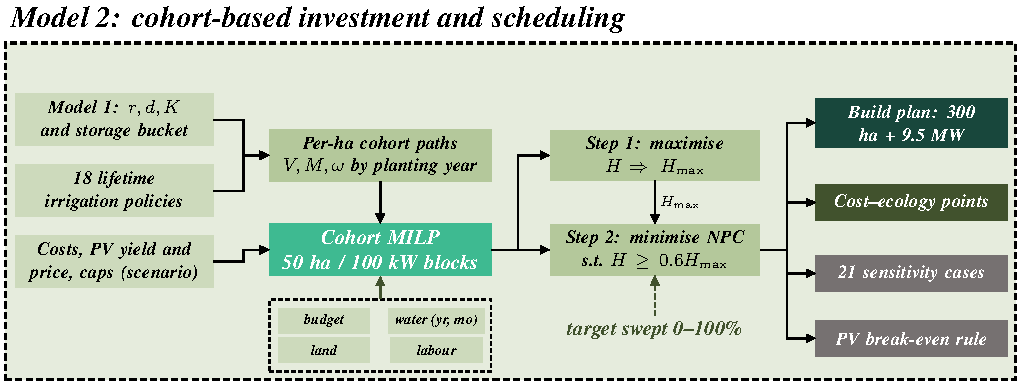
\includegraphics[width=\textwidth]{m2_structure.pdf}
\caption{Structure of Model 2. Model 1 is run once per irrigation policy to get per-hectare paths;
the optimiser then chooses how many 50 ha blocks of each (planting year, policy) cohort and how many 100 kW PV blocks to build.}
\label{fig:struct}
\end{figure}

\begin{enumerate}
\item \textbf{Cohorts.} A cohort $j=(s,p)$ is land planted in year $s$ that follows lifetime irrigation policy $p$.
All land of one cohort has the same state $(V,M)$, so area only scales its water, cost, labour and ecology.
\item \textbf{Policy library (18 policies).} Constant 0, 100, 300, 600, 1,000 mm/yr; switch policies
(100$\to$300, 100$\to$600, 300$\to$600, 600$\to$300, 1,000$\to$600, 300$\to$100) after age 3 or 5;
and a ramp 100 (ages 1--3) $\to$ 300 (ages 4--7) $\to$ 600 mm/yr (age 8+). Rising and falling schedules are both allowed.
\item \textbf{Precompute.} Model 1 is run for each policy from $V_0=2\%$, $M_0=37.5$ mm, giving per-hectare
$V$, $M$, $\omega$ (met-demand ratio) and water by age.
\item \textbf{MILP.} Because cohorts do not share soil water, every quantity is linear in the number of blocks:
a mixed-integer linear programme over 15 years (SciPy \texttt{milp}/HiGHS, gap tolerance 0.2\%, 30 s per solve).
\item \textbf{Two steps.} (i) maximise ecology $H$ to get $H_{\max}$; (ii) minimise net present cost with $H\ge\varphi H_{\max}$, $\varphi=0.6$.
Sweeping $\varphi=0,0.2,\dots,1$ gives the cost--ecology points.
\end{enumerate}

\paragraph{Timing within a year.} Planting and PV construction are paid at the start of the year;
upkeep, water and PV income at the end. New PV earns from the \emph{next} year. Ecology in year $t$ uses the
cover at the start of that year. Ecology land and PV land do not overlap.

\say{Explain why cohorts are needed: a single ``total area'' state cannot tell a new stand from a mature one,
and new stands need years to reach full cover and keep needing water.}

% =====================================================================
\section{Formulas and what they mean}

\subsection{Decisions and stocks}
\begin{align}
a_{sp}&=\Delta_A n_{sp},\quad y_s=\Delta_P z_s,\quad n_{sp},z_s\in\mathbb Z_{\ge0} &&\text{area and PV built, in blocks}\label{eq:blocks}\\
A_t&=\textstyle\sum_{s\le t,p}a_{sp},\quad a_t=\sum_pa_{tp} &&\text{area in service; new area}\\
P_t^{\rm inst}&=\textstyle\sum_{s\le t}y_s,\quad P_t^{\rm op}=\sum_{s<t}y_s &&\text{PV installed; PV producing}
\end{align}

\subsection{Link to Model 1 (each cohort)}
\begin{align}
(M_{sp,t+1},\ \omega_{sp,t})&=\mathcal W\big(V_{sp,t},M_{sp,t},q_{p,t-s}\big)\label{eq:bucket}\\
V_{sp,t+1}&=V_{sp,t}+rV_{sp,t}(1-V_{sp,t}/K)\,\omega_{sp,t}-dV_{sp,t}-kE(1-\eta V_{sp,t}/K)V_{sp,t}\label{eq:veg}
\end{align}
$\mathcal W$ is the Model 1 storage bucket run over one year with quota $q_{p,h}$ (mm/yr) at stand age $h=t-s$;
$\omega$ is the share of transpiration demand met. Parameters are those of Model 1 ($r=0.547$, $d=0.107$, $K=38.08\%$, $k=0$).

\subsection{Ecology objective}
\begin{equation}\label{eq:H}
H=\sum_{t}\sum_{s\le t,p}a_{sp}\,\frac{V_{sp,t}}{K}\qquad[\text{effective ha}\cdot\text{yr}]
\end{equation}
One hectare at full local cover ($V=K$) for one year counts as 1. It rewards both area and how green the area is,
and it counts every year, so early planting is worth more.

\subsection{Water, money, labour and PV}
\begin{align}
Q_t^e&=10\textstyle\sum_{s\le t,p}a_{sp}\,q_{p,t-s},\qquad Q_t=Q_t^e+w_cP_t^{\rm op} &&\text{gross water (m$^3$); 1 mm on 1 ha = 10 m$^3$}\label{eq:water}\\
C_t^b&=c_ba_t,\qquad C_t^p=c_py_t &&\text{planting and PV construction}\\
C_t^o&=c_mA_t+c_{pm}P_t^{\rm op}+c_wQ_t &&\text{upkeep of all stands, PV O\&M, water}\\
D_t&=C_t^b+C_t^o+C_t^p,\qquad (f_t^b,f_t^o,f_t^p)=(C_t^b,C_t^o,C_t^p)/D_t &&\text{spending and its three shares}\label{eq:shares}\\
L_t&=\ell_ba_t+\ell_mA_t+\ell_py_t+\ell_{pm}P_t^{\rm op} &&\text{labour (person-days)}\label{eq:labour}\\
G_t&=\textstyle\sum_{s<t}y_se_0(1-d_p)^{t-s-1},\qquad R_t=p_eG_t &&\text{PV energy (kWh) and income}\label{eq:pv}
\end{align}
Monthly water $Q_{t,m}$ splits each stand's quota by Model 1's monthly demand weights; PV cleaning water is spread evenly over 12 months.

\subsection{Constraints}
\begin{align}
&D_t\le B_t,\qquad \textstyle\sum_tD_t\le B_{\rm tot} &&\text{annual and total budget (income not added back)}\label{eq:budget}\\
&Q_t\le Q^{\max},\qquad Q_{t,m}\le Q_m^{\max}\ (m=1,\dots,12) &&\text{annual and monthly water}\\
&A_t+\alpha_pP_t^{\rm inst}\le A^{\max},\quad a_t\le a^{\max},\quad P_t^{\rm inst}\le P^{\max} &&\text{land, build rate, grid capacity}\\
&L_t\le L^{\max} &&\text{labour}\label{eq:lab}\\
&\underline f_p\textstyle\sum_tD_t\le\sum_tC_t^p\le\overline f_p\sum_tD_t &&\text{optional PV share of total spending}
\end{align}

\subsection{Cost objective and trade-off}
\begin{equation}\label{eq:npc}
N=\sum_{t=0}^{T-1}\Big[\delta^t\big(C_t^b+C_t^p\big)+\delta^{t+1}\big(C_t^o-R_t\big)\Big],\qquad \delta=\frac1{1+0.05}
\end{equation}
\begin{equation}\label{eq:eps}
\text{Step 1: }H_{\max}=\max H\quad\text{s.t. constraints};\qquad
\text{Step 2: }\min N\quad\text{s.t. } H\ge\varphi H_{\max},\ \text{constraints}.
\end{equation}
The target share $\varphi$ is the explicit weight between ecology and cost (0.6 in the base case). Ecology is not converted into money.
All sensitivity runs keep the same absolute target (1,258.22 effective ha$\cdot$yr), so no case looks cheaper by doing less.

\subsection{PV break-even rule}
\begin{equation}\label{eq:be}
p_e\ \ge\ p_e^{\rm BE}(s)=\frac{c_p+\sum_{t=s+1}^{T-1}\delta^{t+1-s}\,(c_{pm}+c_ww_c)}{\sum_{t=s+1}^{T-1}\delta^{t+1-s}\,e_0(1-d_p)^{t-s-1}}
\end{equation}
Price per kWh at which 1 kW built in year $s$ pays back its own cost within the horizon. Necessary for a standalone PV block,
not sufficient for the whole plan (it ignores competition for budget, land and water).

% =====================================================================
\section{Algorithms}\label{sec:alg}

Model 2 is solved in three stages: build the problem from Model 1 (Alg.~\ref{alg:build}),
solve it with the two-step $\varepsilon$-constraint method (Alg.~\ref{alg:solve}), and check every
answer by replaying it through Model 1 (Alg.~\ref{alg:replay}). Formulas refer to Section~3 and to
Section~4 of \texttt{Reports/model\_v7/model\_v7.tex}.

\begin{algorithm}[H]
\caption{Build the cohort MILP}\label{alg:build}
\begin{algorithmic}[1]
\Require scenario parameters (Table~\ref{tab:par}); Model 1 $r,d,K$, bucket parameters, monthly climatology; policy library $\mathcal P$ (18 policies)
\Ensure matrix $\bm A$, limits $\bm b$, ecology vector $\bm h$, cost vector $\bm n$, integer upper bounds
\For{each policy $p\in\mathcal P$}
  \State Run Model 1 (Alg.~3 of the M1 brief, year after year) for $T$ years from $V_0=2\%$, $M_0=37.5$ mm
  \State Store per hectare and by stand age: $V_{\rm start}$, irrigation (mm), monthly gross irrigation
\EndFor
\For{each start year $s=1,\dots,T$}
  \For{each policy $p$} \Comment{drop policies identical over the remaining $T-s+1$ years}
    \State Column ``ecology $(s,p)$'' = one 50 ha block; fill year by year: new area, area in service,
    land, planting cost, upkeep $+$ water cost, water (yearly, monthly), labour, effective ha $=50\,V_{\rm start}/K$
  \EndFor
  \If{$s<T$} \Comment{PV built in the last year earns nothing}
    \State Column ``PV $s$'' = one 100 kW block: capex in year $s$; from $s+1$: energy $e_0(1-d_p)^{\rm age}$, income, O\&M, cleaning water, labour; land from $s$
  \EndIf
\EndFor
\State $\bm n\gets$ discounted cost per column (capex at start of year, O\&M and income at end), Eq.~\eqref{eq:npc}
\State $\bm h\gets$ sum over years of effective ha per column, Eq.~\eqref{eq:H}
\State Rows of $\bm A\bm z\le\bm b$: total budget; PV share bounds; for each year: budget, water, land, new area, labour, PV capacity; for each year and month: water
\State Integer bounds: ecology $\le\lfloor\min(200,1200)/50\rfloor$ blocks, PV $\le10{,}000/100$ blocks
\end{algorithmic}
\end{algorithm}
\noindent\textit{Code:} \texttt{Code/v7\_m2\_core.py} (\texttt{policy\_library}, \texttt{simulate\_policy}, \texttt{build\_problem}).

\begin{algorithm}[H]
\caption{Two-step $\varepsilon$-constraint solution, trade-off points and sensitivity}\label{alg:solve}
\begin{algorithmic}[1]
\Require problem from Alg.~\ref{alg:build}; target share $\varphi=0.6$; gap 0.2\%; time limit 30 s per solve
\Ensure base plan, $H_{\max}$, six trade-off points, 21 sensitivity plans
\State \textbf{Step 1:} $\bm z^{\max}\gets\arg\max\ \bm h^\top\bm z$ s.t.\ $\bm A\bm z\le\bm b$, $\bm z\in\mathbb Z_{\ge0}$;\quad $H_{\max}\gets\bm h^\top\bm z^{\max}$
\State \textbf{Step 2:} $\bm z^*\gets\arg\min\ \bm n^\top\bm z$ s.t.\ $\bm A\bm z\le\bm b$, $\bm h^\top\bm z\ge\varphi H_{\max}$ \Comment{base plan}
\For{each solve}
  \State Call the MILP solver (HiGHS through SciPy \texttt{milp}); record status, objective, bound and gap
  \State If no feasible plan: report ``infeasible'' and stop for this case (no made-up answer)
  \State Round $\bm z$ and check integrality ($10^{-4}$) and every constraint ($10^{-7}$) independently
\EndFor
\For{$\varphi\in\{0,0.2,0.4,0.6,0.8,1.0\}$}
  \State Solve Step 2 with target $\varphi H_{\max}$ \Comment{Table~\ref{tab:front}}
\EndFor
\For{each sensitivity case (one parameter changed)}
  \State Rebuild the problem (Alg.~\ref{alg:build}); solve Step 2 with the \emph{same} target $0.6H_{\max}=1{,}258.22$ \Comment{Table~\ref{tab:sens}}
\EndFor
\State For each build year $s$: compute the PV break-even price, Eq.~\eqref{eq:be}, and standalone NPV \Comment{Table~\ref{tab:pv}}
\end{algorithmic}
\end{algorithm}
\noindent\textit{Code:} \texttt{Code/v7\_m2\_core.py} (\texttt{solve}), \texttt{Code/v7\_model2.py} (\texttt{run}).

\begin{algorithm}[H]
\caption{Replay check of a solved plan}\label{alg:replay}
\begin{algorithmic}[1]
\Require chosen block counts $\bm z^*$
\Ensure yearly and monthly ledgers; largest difference from the MILP rows
\For{each chosen ecology cohort $(s,p)$ with area $a$}
  \State Re-run Model 1 for policy $p$ from year $s$ to $T$ (not the cached columns)
  \State Add its area, water (yearly, monthly), upkeep, labour, effective ha to the yearly ledger
\EndFor
\For{each chosen PV block}
  \State Add capex, energy, income, O\&M, cleaning water, land, labour by year
\EndFor
\State Compute fund shares $(f^b_t,f^o_t,f^p_t)$, budget left, discounted net cost
\State Compare every ledger column with $\bm A\bm z^*$, $\bm h^\top\bm z^*$, $\bm n^\top\bm z^*$; base case largest difference $1.9\times10^{-9}$
\end{algorithmic}
\end{algorithm}
\noindent\textit{Code:} \texttt{Code/v7\_m2\_core.py} (\texttt{replay}). Run: \texttt{python Code/v7\_model2.py};
tests: \texttt{python -m unittest discover -s Code -p test\_v7\_m2.py} (7 tests, incl.\ brute-force check on a small case).

\say{Explain in the paper why the problem is linear although Model 1 is not: Model 1 is run once per policy
before optimising, and cohorts do not share soil water, so every cost, water and ecology term is the per-block
value times the number of blocks.}

% =====================================================================
\section{Parameters}

\begin{table}[H]\centering\small
\begin{tabularx}{\textwidth}{@{}>{\raggedright\arraybackslash}p{4.3cm} >{\raggedright\arraybackslash}p{5.2cm} Y@{}}
\toprule
Parameter & Base value & Source / status\\
\midrule
Horizon $T$ & 15 years & within the recommended 10--20 years\\
Blocks $\Delta_A$, $\Delta_P$ & 50 ha; 100 kW & numerical grid (25 ha also tested)\\
New stand $V_0$, $M_0$ & 2\%; 37.5 mm & assumption (1\% and 4\% tested)\\
Total / annual budget $B_{\rm tot}$, $B_t$ & 80 M; 12 M/yr & planning scenario\\
Land $A^{\max}$; build rate $a^{\max}$ & 1,200 ha; 200 ha/yr & planning scenario\\
Water $Q^{\max}$ & 1.5 M m$^3$/yr & scenario, not a water permit\\
Monthly water $Q^{\max}_m$ (Jan--Dec) & 50, 60, 90, 120, 180, 220, 240, 220, 150, 90, 50, 30 thousand m$^3$ & scenario delivery capacity\\
Labour $L^{\max}$ & 12,000 person-days/yr & scenario\\
Planting cost $c_b$ & 52,500 CNY/ha & Yutian 2024 desert-planting trial (3.5 M for 1,000 mu), transferred; $\pm25\%$ tested\\
Upkeep $c_m$ & 1,500 CNY/(ha$\cdot$yr) & assumption; $\pm50\%$ tested\\
Water price $c_w$ & 1 CNY/m$^3$ & assumption\\
Labour rates $\ell_b$, $\ell_m$ & 30 person-days/ha; 3 per ha$\cdot$yr & assumption\\
PV capex $c_p$; O\&M $c_{pm}$ & 3,000 CNY/kW; 50 CNY/(kW$\cdot$yr) & assumption; 2,250 / 3,750 tested\\
PV net yield $e_0$ & 1,500 kWh/(kW$\cdot$yr) & assumption, net of losses\\
PV price $p_e$ & 0.30 CNY/kWh & scenario; 0.15 / 0.40 tested\\
PV degradation $d_p$ & 0.5\%/yr & Jordan \& Kurtz (2013) median\\
PV land $\alpha_p$; labour $\ell_p$, $\ell_{pm}$ & 0.002 ha/kW; 0.10 and 0.01 person-days/kW & assumption\\
PV cleaning water $w_c$ & 0.02 m$^3$/(kW$\cdot$yr) & assumption\\
PV capacity $P^{\max}$ & 10,000 kW & scenario grid limit\\
Discount rate & 5\%/yr (real) & scenario\\
Ecological target $\varphi$ & 0.60 of $H_{\max}$ & policy choice for the demonstration\\
Model 1 inputs & $r=0.547$, $d=0.107$, $K=38.08\%$, $k=0$, $\eta=1$, $C=75$ mm & from Model 1\\
\bottomrule
\end{tabularx}
\caption{Model 2 parameters. The problem gives no numbers for budget, prices or caps, so all of these are stated assumptions.}
\label{tab:par}
\end{table}

% =====================================================================
\section{Results}

\subsection{Maximum ecology reference}
With every resource devoted to ecology: $H_{\max}=2{,}097.03$ effective ha$\cdot$yr (upper bound 2,098.93, gap 0.09\%),
900 ha planted, no PV, all 80 M spent, net present cost 64.42 M.
The base target is $0.6H_{\max}=1{,}258.22$.

\subsection{Optimal base plan}
\begin{table}[H]\centering\small
\begin{tabular}{@{}llrr@{}}
\toprule
Cohort / asset & Policy (mm/yr by stand age) & Year built & Size\\
\midrule
Ecology A & 100 (ages 1--3) $\to$ 300 & 1 & 100 ha\\
Ecology B & ramp 100 (1--3) $\to$ 300 (4--7) $\to$ 600 (8+) & 1 & 50 ha\\
Ecology C & 100 (ages 1--3) $\to$ 300 & 2 & 150 ha\\
PV & -- & 1 / 2 / 3 / 4 & 1,200 / 1,100 / 3,700 / 3,500 kW\\
\bottomrule
\end{tabular}
\caption{What to build. Total 300 ha and 9,500 kW.}
\label{tab:plan}
\end{table}

\begin{table}[H]\centering\small
\begin{tabular}{@{}lrr@{}}
\toprule
Indicator & Value & Note\\
\midrule
Ecology achieved & 1,264.84 eff.\ ha$\cdot$yr & target 1,258.22\\
Total spending (undiscounted) & 68.93 M & 86\% of 80 M\\
\quad planting / upkeep + water / PV construction & 15.75 / 24.68 / 28.50 M & \\
PV income (undiscounted, 15 yr) & 49.90 M & \\
Net present cost $N$ & 25.35 M & lower bound 25.30 M, gap 0.20\%\\
Without PV (best plan) & 27.84 M & PV saves 2.49 M (9\%)\\
Peak annual water & 1.050 M m$^3$ & 70\% of annual cap\\
Peak monthly water use & 94.9\% of May cap & years 8--15\\
Peak labour & 5,522 person-days & 46\% of cap\\
Land used & 319 ha & of 1,200 ha\\
\bottomrule
\end{tabular}
\caption{Base plan summary.}
\end{table}

\begin{table}[H]\centering\footnotesize
\resizebox{\textwidth}{!}{\begin{tabular}{@{}rrrrrrrrrr@{}}
\toprule
Year & New ha & Stock ha & New PV kW & PV producing kW & Planting M & Upkeep+water M & PV build M & Spending M & PV income M\\
\midrule
1 & 150 & 150 & 1,200 & 0 & 7.88 & 0.38 & 3.60 & 11.85 & 0.00\\
2 & 150 & 300 & 1,100 & 1,200 & 7.88 & 0.81 & 3.30 & 11.99 & 0.54\\
3 & 0 & 300 & 3,700 & 2,300 & 0.00 & 0.87 & 11.10 & 11.97 & 1.03\\
4 & 0 & 300 & 3,500 & 6,000 & 0.00 & 1.35 & 10.50 & 11.85 & 2.69\\
5 & 0 & 300 & 0 & 9,500 & 0.00 & 1.83 & 0.00 & 1.83 & 4.25\\
6 & 0 & 300 & 0 & 9,500 & 0.00 & 1.83 & 0.00 & 1.83 & 4.23\\
7 & 0 & 300 & 0 & 9,500 & 0.00 & 1.83 & 0.00 & 1.83 & 4.21\\
8 & 0 & 300 & 0 & 9,500 & 0.00 & 1.98 & 0.00 & 1.98 & 4.19\\
9 & 0 & 300 & 0 & 9,500 & 0.00 & 1.98 & 0.00 & 1.98 & 4.17\\
10 & 0 & 300 & 0 & 9,500 & 0.00 & 1.98 & 0.00 & 1.98 & 4.15\\
11 & 0 & 300 & 0 & 9,500 & 0.00 & 1.98 & 0.00 & 1.98 & 4.13\\
12 & 0 & 300 & 0 & 9,500 & 0.00 & 1.98 & 0.00 & 1.98 & 4.11\\
13 & 0 & 300 & 0 & 9,500 & 0.00 & 1.98 & 0.00 & 1.98 & 4.09\\
14 & 0 & 300 & 0 & 9,500 & 0.00 & 1.98 & 0.00 & 1.98 & 4.07\\
15 & 0 & 300 & 0 & 9,500 & 0.00 & 1.98 & 0.00 & 1.98 & 4.05\\
\bottomrule
\end{tabular}}
\caption{Base plan, year by year: building and money.}
\label{tab:yearA}
\end{table}

\begin{table}[H]\centering\footnotesize
\begin{tabular}{@{}rrrrcrr@{}}
\toprule
Year & Water (k m$^3$) & Labour (p-d) & Effective ha & Shares build / O\&M / PV & Budget left M & Discounted net cost M\\
\midrule
1 & 150.0 & 5,070 & 7.9 & 0.66 / 0.03 / 0.30 & 68.15 & 11.83\\
2 & 300.0 & 5,522 & 19.0 & 0.66 / 0.07 / 0.28 & 56.16 & 10.89\\
3 & 300.0 & 1,293 & 26.7 & 0.00 / 0.07 / 0.93 & 44.20 & 9.92\\
4 & 600.1 & 1,310 & 35.2 & 0.00 / 0.11 / 0.89 & 32.35 & 7.97\\
5 & 900.2 & 995 & 46.2 & 0.00 / 1.00 / 0.00 & 30.52 & $-$1.90\\
6 & 900.2 & 995 & 62.3 & 0.00 / 1.00 / 0.00 & 28.70 & $-$1.80\\
7 & 900.2 & 995 & 80.5 & 0.00 / 1.00 / 0.00 & 26.87 & $-$1.70\\
8 & 1,050.2 & 995 & 95.1 & 0.00 / 1.00 / 0.00 & 24.90 & $-$1.50\\
9 & 1,050.2 & 995 & 107.5 & 0.00 / 1.00 / 0.00 & 22.92 & $-$1.41\\
10 & 1,050.2 & 995 & 117.2 & 0.00 / 1.00 / 0.00 & 20.95 & $-$1.33\\
11 & 1,050.2 & 995 & 124.6 & 0.00 / 1.00 / 0.00 & 18.97 & $-$1.26\\
12 & 1,050.2 & 995 & 130.2 & 0.00 / 1.00 / 0.00 & 17.00 & $-$1.19\\
13 & 1,050.2 & 995 & 134.5 & 0.00 / 1.00 / 0.00 & 15.02 & $-$1.12\\
14 & 1,050.2 & 995 & 137.8 & 0.00 / 1.00 / 0.00 & 13.05 & $-$1.06\\
15 & 1,050.2 & 995 & 140.3 & 0.00 / 1.00 / 0.00 & 11.07 & $-$1.00\\
\bottomrule
\end{tabular}
\caption{Base plan, year by year: resources, fund shares, ecology. Effective ha $=\sum$ area $\times V/K$; their sum over 15 years is $H$.}
\label{tab:yearB}
\end{table}

\begin{itemize}
\item \textbf{Front-loaded.} Planting and PV fill the 12 M annual budget in years 1--4 (slack 0.15, 0.015, 0.035, 0.15 M); from year 5 only upkeep is paid.
\item \textbf{PV pays for upkeep.} From year 5, PV income (4.05--4.25 M/yr) exceeds all upkeep and water (1.83--1.98 M/yr), so the yearly net cost is negative.
\item \textbf{Water steps up with stand age}: 150 k m$^3$ (year 1) $\to$ 300 k $\to$ 600 k (year 4) $\to$ 900 k (year 5) $\to$ 1,050 k m$^3$ (year 8 on).
\item \textbf{Monthly bottleneck.} Highest monthly use relative to cap: May 94.9\%, April 88.7\%, June 87.3\%, July 86.1\%; the annual total uses only 70\%.
\end{itemize}

\begin{table}[H]\centering\small
\begin{tabular}{@{}lrrrrrr@{}}
\toprule
Cohort & \multicolumn{6}{c}{Cover $V$ at start of project year (\%) [quota mm/yr]}\\
 & 1 & 3 & 5 & 8 & 10 & 15\\
\midrule
A (100 ha, yr 1) & 2.00 [100] & 3.95 [100] & 6.75 [300] & 12.76 [300] & 14.68 [300] & 16.90 [300]\\
B (50 ha, yr 1, ramp) & 2.00 [100] & 3.95 [100] & 6.75 [300] & 12.76 [600] & 18.41 [600] & 23.15 [600]\\
C (150 ha, yr 2) & -- & 2.82 [100] & 4.98 [300] & 11.37 [300] & 13.83 [300] & 16.64 [300]\\
\bottomrule
\end{tabular}
\caption{Cohort trajectories inherited from Model 1 ($K=38.08\%$).}
\end{table}

\subsection{Ecology--cost trade-off}
\begin{table}[H]\centering\small
\resizebox{\textwidth}{!}{\begin{tabular}{@{}rrrrrrr@{}}
\toprule
Target $\varphi$ & $H$ achieved & Net present cost M & Spending M & Area ha & PV kW & Marginal cost (k CNY per eff.\ ha$\cdot$yr)\\
\midrule
0\% & 0 & $-$4.91 & 36.60 & 0 & 10,000 & --\\
20\% & 428.05 & 4.78 & 49.22 & 100 & 10,000 & 22.6\\
40\% & 839.97 & 14.17 & 58.72 & 150 & 10,000 & 22.8\\
60\% & 1,264.84 & 25.35 & 68.93 & 300 & 9,500 & 26.3\\
80\% & 1,678.79 & 40.52 & 70.59 & 500 & 5,300 & 36.7\\
100\% & 2,097.03 & 64.42 & 80.00 & 900 & 0 & 57.1\\
\bottomrule
\end{tabular}}
\caption{Six solved points (not a fitted curve). Marginal cost = change in $N$ / change in $H$ from the previous row.}
\label{tab:front}
\end{table}
\begin{itemize}
\item Cost rises faster than ecology: the marginal cost per effective ha$\cdot$yr is flat to 40\%, then rises 2.5-fold by 100\%.
\item As the target rises, PV is pushed out (10 MW $\to$ 0) because budget is needed for planting and upkeep.
\item With no ecological requirement, PV alone earns 4.91 M in present value; this is not a reason to skip treatment.
\end{itemize}

\subsection{Sensitivity (same absolute target 1,258.22)}
\begin{table}[H]\centering\small
\begin{tabular}{@{}lrrrrr@{}}
\toprule
Case & $N$ (M) & Change vs base & Area ha & PV kW & MIP gap \%\\
\midrule
Base & 25.35 & -- & 300 & 9,500 & 0.20\\
\midrule
No PV allowed & 27.84 & +9.8\% & 300 & 0 & 0.04\\
PV price 0.15 CNY/kWh & 27.84 & +9.8\% & 300 & 0 & 0.04\\
PV price 0.40 CNY/kWh & 14.28 & $-$43.7\% & 300 & 10,000 & 0.10\\
PV capex 2,250 CNY/kW & 17.76 & $-$30.0\% & 300 & 10,000 & 0.00\\
PV capex 3,750 CNY/kW & 27.84 & +9.8\% & 300 & 0 & 0.04\\
PV share of spending $\ge10\%$ & 25.35 & 0.0\% & 300 & 9,500 & 0.20\\
PV share of spending $\ge30\%$ & 25.35 & 0.0\% & 300 & 9,500 & 0.20\\
O\&M $-50\%$ (750 /ha, 25 /kW) & 21.21 & $-$16.3\% & 300 & 10,000 & 0.17\\
O\&M $+50\%$ (2,250 /ha, 75 /kW) & 29.09 & +14.8\% & 300 & 5,600 & 0.13\\
Planting cost 39,375 CNY/ha & 20.86 & $-$17.7\% & 300 & 10,000 & 0.08\\
Planting cost 65,625 CNY/ha & 29.93 & +18.1\% & 300 & 8,000 & 0.18\\
Water caps $-20\%$ & 27.82 & +9.7\% & 350 & 8,500 & 0.20\\
Water caps $+10\%$ & 24.99 & $-$1.4\% & 300 & 9,500 & 0.20\\
Total budget 64 M & 25.45 & +0.4\% & 300 & 8,100 & 0.14\\
Labour cap 6,000 & 25.35 & 0.0\% & 300 & 9,500 & 0.13\\
Initial cover 1\% & 32.74 & +29.1\% & 400 & 7,500 & 0.19\\
Initial cover 4\% & 20.42 & $-$19.5\% & 200 & 10,000 & 0.19\\
Area block 25 ha & 25.29 & $-$0.2\% & 300 & 9,400 & 0.20\\
Storage capacity 37.5 mm & 25.79 & +1.7\% & 300 & 9,300 & 0.20\\
Storage capacity 150 mm & 25.14 & $-$0.8\% & 300 & 9,400 & 0.20\\
Constant-quota policies only & 27.04 & +6.6\% & 300 & 8,800 & 0.00\\
\bottomrule
\end{tabular}
\caption{One-at-a-time sensitivity. Differences below about 0.4\% are within solver tolerance.}
\label{tab:sens}
\end{table}
\begin{itemize}
\item \textbf{PV is all-or-nothing on price.} At 0.15 CNY/kWh or 3,750 CNY/kW no PV is built; at 0.40 CNY/kWh or 2,250 CNY/kW the full 10 MW is built and cost falls 30--44\%.
\item \textbf{Establishment success matters most among ecology inputs}: initial cover 1\% vs 4\% moves cost by +29\% / $-$20\% and needs 400 vs 200 ha.
\item Upkeep and planting prices move cost by 15--18\% for $\pm$25--50\%.
\item Labour and the budget are not binding at this target; water binds when caps are cut by 20\% (the plan changes to 350 ha and 8.5 MW, +9.7\%).
\item Allowing rising/falling schedules saves 6.6\% versus constant quotas only.
\end{itemize}

\subsection{PV screening by construction year}
\begin{table}[H]\centering\small
\begin{tabular}{@{}lrrrrrrrr@{}}
\toprule
Build year & 1 & 2 & 3 & 4 & 5 & 6 & 8 & 10\\
\midrule
Break-even price (CNY/kWh) & 0.253 & 0.264 & 0.277 & 0.293 & 0.312 & 0.335 & 0.402 & 0.523\\
Standalone NPV (CNY/kW) & 652 & 473 & 284 & 85 & $-$126 & $-$348 & $-$830 & $-$1,368\\
\bottomrule
\end{tabular}
\caption{At the base price 0.30 CNY/kWh, PV pays for itself only if built in years 1--4, which are exactly the years the optimiser chose.}
\label{tab:pv}
\end{table}

\subsection{Verification}
29 optimisation runs, all feasible, all gaps $\le0.20\%$. Every plan is replayed through Model 1 and every
ledger (money, water, labour, land, PV) is recomputed: largest difference $1.9\times10^{-9}$.
7 unit tests, including a brute-force check of all integer plans on a small instance against the MILP answer.

% =====================================================================
\section{Actionable process criteria}\label{sec:rules}
\begin{enumerate}
\item \textbf{PV entry rule.} Build a PV block in year $s$ only if the expected price satisfies Eq.~\eqref{eq:be},
$p_e\ge p_e^{\rm BE}(s)$ (base: 0.253 in year 1 rising to 0.312 in year 5), \emph{and} the plan still meets the budget,
monthly water and land limits. Under base prices this means PV only in years 1--4.
\item \textbf{Water follows stand age.} Give new stands about 100 mm/yr (1,000 m$^3$/ha) for the first three years and
raise to 300 mm/yr from year 4; a share of the area can go to 600 mm/yr from year 8 to lift cover further.
Young stands use little water: in Model 1, quotas above about 300 mm/yr give no extra growth in the first five years (the surplus drains), and the optimiser found 100 mm/yr cheapest for the first three.
\item \textbf{Plant early.} Put all planting in the first two years (as fast as the annual budget allows), since every
year of growing cover adds to the ecological total and stands need 10--15 years to approach their plateau.
\item \textbf{Check months, not only years.} Schedule water against the May, April and June caps; they bind long before the annual total.
\item \textbf{Choose the target where the cost curve bends.} Up to 40--60\% of the maximum, each effective ha$\cdot$yr costs 23--26 k CNY;
above 80\% it costs 57 k CNY. Raise the target only if that price is acceptable.
\item \textbf{Measure establishment first.} Initial cover is the input that changes cost most; a pilot survival survey is the most valuable data to collect.
\end{enumerate}

% =====================================================================
\section{What we can claim and what we cannot}
\begin{tabularx}{\textwidth}{@{}YY@{}}
\toprule
Can claim & Must not claim\\
\midrule
A dynamic plan that tracks every cohort's vegetation and soil water and respects budget, water (yearly and monthly), land and labour. &
That 300 ha and 9.5 MW is a recommended project size; budget, caps and prices are assumptions. \\
Optimality within the 18-policy library and 50 ha grid, with gap $\le0.2\%$. &
Global optimum over all possible watering schedules or continuous areas. \\
PV is worth building only early and only above the break-even price; it can finance upkeep. &
That more PV is always better, or a guaranteed PV income. \\
Rising marginal cost of ecology; the monthly water cap is the bottleneck. &
That $H$ is a measured ecological benefit, erosion reduction or money value. \\
\bottomrule
\end{tabularx}

% =====================================================================
\section{Figures ready for the paper}
\begin{table}[H]\centering\small
\begin{tabularx}{\textwidth}{@{}lY@{}}
\toprule
File (\texttt{Figures/M2/}) & What it shows / caption point\\
\midrule
\texttt{m2\_f01\_build\_and\_spending} & New and stock area; PV built and producing; three spending streams vs annual budget; spending shares\\
\texttt{m2\_f02\_cohorts} & Cover, quota and storage of the three cohorts; their contribution to effective area\\
\texttt{m2\_f03\_water\_pressure} & Annual and monthly water vs caps; month-by-year use of the cap\\
\texttt{m2\_f04\_cost\_ecology\_points} & Six solved trade-off points; area, PV and MIP gap at each\\
\texttt{m2\_f05\_investment\_sensitivity} & Cost, PV and spending mix under price, cost and PV-share cases\\
\texttt{m2\_f06\_assumption\_checks} & Initial cover, storage, caps, grid, constant-only policies\\
\texttt{m2\_f07\_pv\_screening} & Break-even price and standalone NPV by build year\\
\bottomrule
\end{tabularx}
\end{table}

\begin{figure}[H]\centering
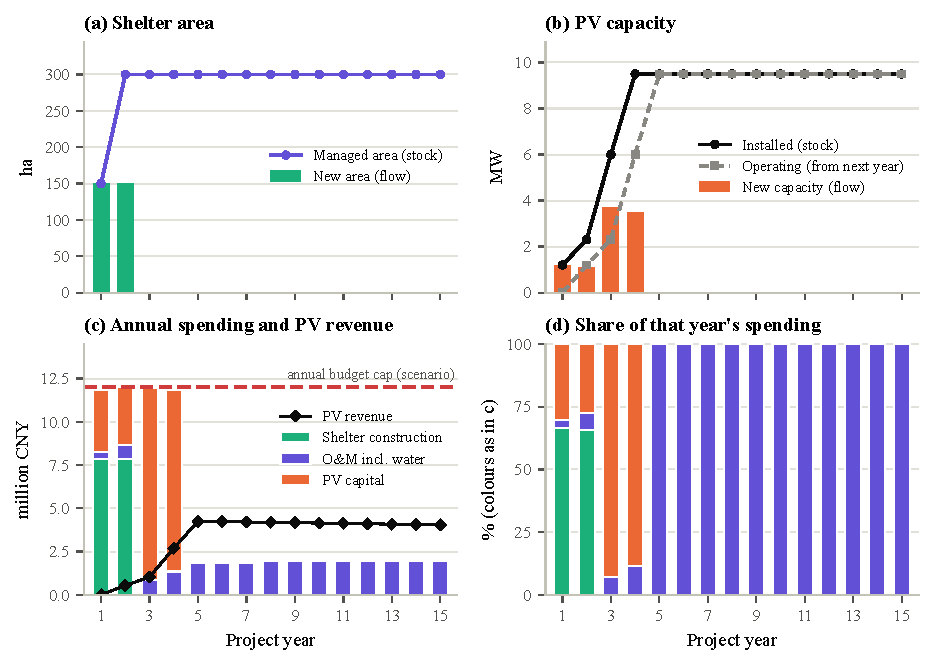
\includegraphics[width=0.92\textwidth]{../../Figures/M2/m2_f01_build_and_spending.pdf}
\caption{(From \texttt{m2\_f01}) Base plan: building, PV and spending by year.}
\end{figure}

\begin{figure}[H]\centering
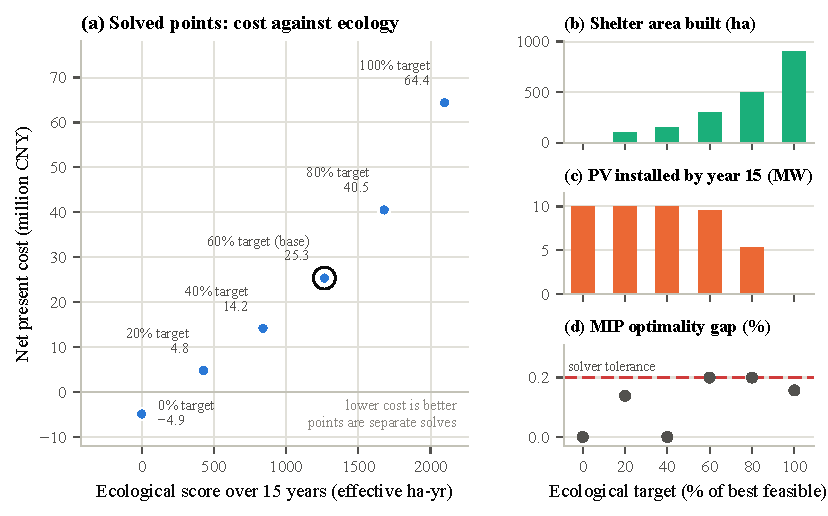
\includegraphics[width=0.92\textwidth]{../../Figures/M2/m2_f04_cost_ecology_points.pdf}
\caption{(From \texttt{m2\_f04}) Ecology--cost trade-off at six solved targets.}
\end{figure}

\section{Suggested outline for the Model 2 section}
\begin{enumerate}
\item Why cohorts: link to Model 1 states; Fig.~\ref{fig:struct}.
\item Decision variables (area, water, three fund shares, labour) and Eqs.~\eqref{eq:blocks}--\eqref{eq:pv}.
\item Constraints \eqref{eq:budget}--\eqref{eq:lab} and the $\varepsilon$-constraint objective \eqref{eq:npc}--\eqref{eq:eps}.
\item Algorithms: build (Alg.~\ref{alg:build}), two-step solve (Alg.~\ref{alg:solve}), replay check (Alg.~\ref{alg:replay}).
\item Parameters (Table~\ref{tab:par}) with the note that they are scenario values.
\item Base plan (Tables~\ref{tab:plan}--\ref{tab:yearB}) and the trade-off (Table~\ref{tab:front}).
\item Sensitivity of the investment structure (Table~\ref{tab:sens}) and PV screening (Table~\ref{tab:pv}).
\item Actionable criteria (Section~\ref{sec:rules}) and limits.
\end{enumerate}

\end{document}
